\documentclass{bmvc2k}

%% Enter your paper number here for the review copy
\bmvcreviewcopy{??}

\usepackage{amsfonts,amssymb} 
\usepackage{subfigure}
\usepackage{booktabs}
\usepackage{diagbox}
\usepackage{graphicx}
\usepackage{multirow}


\title{3D Object Detection and Tracking in Streaming Data}

% Enter the paper's authors in order
% \addauthor{Name}{email/homepage}{INSTITUTION_CODE}
\addauthor{Xusen Guo}{guoxs3@mail2.sysu.edu.cn}{1}
\addauthor{Kai Huang}{huangk36@mail.sysu.edu.cn}{1}

% Enter the institutions
% \addinstitution{Name\\Address}
\addinstitution{
	Key Laboratory of Machine Intelligence\\
	and Advanced Computing, Ministry of \\
	Education School of Data and Computer Science, Sun Yat-Sen \\
	University, GuangZhou, China
}

\runninghead{XuSen Guo, KaiHuang, SYSU}{3D Object Detection and Tracking in Streaming Data}

% Any macro definitions you would like to include
% These are not defined in the style file, because they don't begin
% with \bmva, so they might conflict with the user's own macros.
% The \bmvaOneDot macro adds a full stop unless there is one in the
% text already.
\def\eg{\emph{e.g}\bmvaOneDot}
\def\Eg{\emph{E.g}\bmvaOneDot}
\def\etal{\emph{et al}\bmvaOneDot}

%-------------------------------------------------------------------------
% Document starts here
\begin{document}
\maketitle
\begin{abstract}
Recent approaches for 3D object detection have made great progresses due to the evolution in deep learning. However, previous works are mostly based on single frame point cloud or image, information between frames is scarcely explored. In this paper, we try to leverage the temporal information in streaming data and explore 3D object detection and tracking based on multi-frame. Towards this goal, we set up a ConvNet architecture that can associate multi-frame image and LiDAR data to produce accurate 3D detection boxes and trajectories in an end-to-end form. Specially, a correlation module is introduced to capture objects co-occurrences across time, and a multi-task objective for frame-based object detection and across-frame track regression is used. Therefore, the network can perform 3D object detection and tracking simultaneously. Our proposed architecture is shown to produce competitive results on the KITTI Object tracking datasets. Code and models will be available soon.
\end{abstract}

%-------------------------------------------------------------------------
\section{Introduction}
\label{sec:intro} 
Object detection in 2D images has made tremendous progress due to the emergence of deep learning \cite{krizhevsky2012imagenet, simonyan2014very, he2016deep} and their region based descendants \cite{dai2016r, girshick2015fast, ren2015faster} recently. However, extending 2D approaches to 3D scenes is extremely hard because of the increased computational cost and the difficulties in acquiring 3D data. Even though, many work has been carried out inspired by the rapid development of autonomous driving industry. 

Recent approaches in 3D object detection are usually done in three fronts: image based, point cloud based and fusion of image and point cloud. These methods have achieved decent performance but are limited to single frame input. Note that streaming data is more natural and straightforward for most driving scenarios, thus fast and accurate 3D object detection in streaming data is crucial for autonomous driving. However, applying existing single frame based approaches directly to streaming data will inevitably loss the consistency and diversity between frames, and also introduce unaffordable computational cost and time for most applications. Therefore, exploring 3D object detection network specifically for streaming data is valuable and important.

Similar to extend 2D object detection methods to 3D scenes, we can also try to extend video-based object detection approaches to streaming-based 3D object detection. Most modern computer vision approaches to video object detection based on image and require flow estimation, for example, a series work in \cite{zhu2017flow,zhu2018towards} associates vision feature and optical flow to build an accurate end-to-end learning framework for video object detection. However, performing video-based approach for 3D streaming object detection in autonomous driving will be awful, since video suffers from motion blur and partial occlusion, which are conventional in driving scenarios. While another choice is to use LiDAR data, since point cloud provides an accurate spatial representation of the world allowing for precise positioning of objects of interest, thus motion blur and occlusion problem can be avoided in three-dimensional perspective. However, LiDAR does not capture appearance well when compared to the richness of images, additionally, accurate 3D scene flow estimation from point cloud is tremendously tough. Although some approaches such as \cite{liu2018learning, behl2018pointflownet} have been presented to learn 3D motion field in the world, their performance are limited in large and complex scenes. 

Inspired by \cite{feichtenhofer2017detect}, we transform AVOD \cite{ku2018joint} structure into 
a dual-way network embedding with a correlation module, named Bi-AVOD, which takes two adjacent key frames as input and predicts location and orientation of object as well as their local displacement. Note that Bi-AVOD is an aggregate view object detection architecture capable of fusing different features in image and point cloud, thus its input includes two adjacent images in front view and two adjacent BEV (bird eye view) from LIDAR data. While the correlation module compute convolutional cross-correlation between the features response of adjacent key frames to estimate displacement of the same objects. With local displacement and object orientation, object location in intermediate frames can be calculated by interpolation. Moreover, object detection boxes can be linked between frames with the help of local displacement, then multiple object tracking can be performed through \textit{tracking by detection} \cite{lenz2015followme}. 

In summary, our contributions are threefold: \textit{(i)} we set up a two stream architecture based on AVOD for simultaneous 3D streaming object detection and tracking; \textit{(ii)} we introduce correlation module to capture object co-occurrences across time and perform frame-level 3D object detection in a high speed through interpolation; \textit{(iii)} we utilize tracking result to improve detection performance and preliminary explore the scheme of key frame selection. 
%-------------------------------------------------------------------------
\section{Related Work}
\label{sec:related work}

\subsection{3D object detection}
Currently, most approaches in 3D object detection can be divided into three types: image based detectors, LiDAR based detectors and fusion based detectors. Image based approaches such as Mono3D \cite{7780605}, 3DOP \cite{chen20183d} use camera data only, since images are limited in depth information, specific hand-crafted geometric features are required. LiDAR based methods are usually done in two fronts, one is utilizing a voxel grid representation to encoder point cloud and then applying 3D CNN for features extracting, these approaches including 3D FCN \cite{li20173d}, Vote3Deep \cite{engelcke2017vote3deep} and VoxelNet \cite{zhou2018voxelnet} \etal These approaches suffer from the sparsity of point cloud and enormous computation cost in 3D convolution. While others try to project point cloud to bird eye view (BEV) and apply 2D CNN for object detection, such as PIXOR \cite{yang2018pixor}, FaF \cite{luo2018fast} and Comple-YOLO \cite{simon2018complex} \etal These methods take advantage of the fact that 3D detections in driving scenes almost on the same plane thus loss of height information has little affect to the performance, while the depth and geometric information can be retained and computational complexity reduced significantly, making real-time detection possible. However, due to the sparsity of point cloud, the feature information after projecting is insufficient for accurate object detection especially for small targets.

There are also many multi-modal fusion methods that combine image and LiDAR data to improve detection accuracy. F-PointNet \cite{qi2018frustum} first extracts the 3D bounding frustum of an object by extruding 2D bounding boxes from image detectors, then consecutively perform 3D object instance segmentation and amodal extent regression to estimate the amodal 3D bounding box. MV3D \cite{chen2017multi} extends the image based RPN of Faster R-CNN\cite{ren2015faster} to 3D and proposes a 3D RPN targeted in autonomous driving scenarios. MV3D uses every pixel in BEV feature map to multiple 3D anchors and then feeds the anchor to RPN to generate 3D proposals that are used to create view-specific feature crops from BEV feature maps and images. Then a deep fusion scheme is used to combine information from these feature crops to produce final detection output. However, MV3D does not work well for small targets due to the insufficient data for feature extracting caused by downsampling in convolutional feature extractors. AVOD \cite{ku2018joint} architecture is similar to MV3D in 3D RPN and feature fusion, however, its feature extraction module provides full resolution feature maps that leading great improvement in localization accuracy for small targets. In our proposed architecture, AVOD framework is used for basic 3D object detection module.

\subsection{Video object detection}
Video object detection has received increasing attention since ImageNet VID datasets introduced. In this challenge, nearly all of existing methods incorporate temporal information on either final box level or feature level. T-CNN \cite{kang2018t, kang2016object} leverages precomputed optical flows to propagate predicted bounding box to neighboring frames, and then generates tubelets by applying tracking algorithms from high-confidence bounding boxes. Seq-NMS \cite{han2016seq} improves NMS algorithm for video by constructing sequences along nearby high-confidence bounding boxes from consecutive frames, then boxes of the sequence are re-scored to the average confidence and other boxes close to this sequence are suppressed. 

FGFA \cite{zhu2017flow} leverages temporal coherence on feature level, it first applies feature extraction network on individual frames to produce the per-frame feature maps, and then enhance the features at a reference frame by warping the nearby frames feature maps according to the flow emotion, and then the detection network performs object detection only on the reference frame. Later a more efficient approach based on FGFA has been presented in \cite{zhu2018towards}, it introduces three new techniques, sparsely recursive feature aggregation, spatially-adaptive partial feature updating and temporally-adaptive key frame scheduling, which make this unified approach faster, more accurate and more flexible.

There are also some approaches try to learn temporal information between consecutive frames during network training. D\&T \cite{feichtenhofer2017detect} presents an fully convolutional architecture end-to-end using a detection and tracking based loss for simultaneous detection and tracking in video. In order to learn temporal information representation, the network is fed with multiple frames and a correlation module is embedded for computing convolutional cross-correlation between these frames feature maps. Our Bi-AVOD approach mainly inspired by this work. 

\subsection{3D multi-object tracking}
3D multi-object tracking is mostly implemented based on tracking by detection. For example, FaF \cite{luo2018fast} jointly reasons about 3D detection, tracking and motion forecasting taking a 4D tensor created from multiple consecutive temporal frames. DSM \cite{frossard2018end} first predicts 3D bounding boxes in continuous frames and then data association using a Matching net and Scoring net, which is similar to our approach. However, their 3D detector is based on MV3D but ours is AVOD, and their bounding boxes association is done by solving a linear program while ours simply uses a extending IOU based algorithm \cite{bochinski2018extending} in 3D with the help of corresponding displacements over time.
%-------------------------------------------------------------------------
\section{Methodology}
\label{sec:method}
In this section we first give an overview of our Bi-AVOD approach (Sect. 3.1) that generates object detection results and tracklets given two adjacent key frames as input. We then introduce the correlation module (Sect. 3.2) that predicts offsets of corresponding targets in two adjacent key frames. Sect. 3.3 shows the multi-task objective function and Sect. 3.4 shows how we implement 3D streaming detection and tracking using prediction results of Bi-AVOD.

\begin{figure}
	\rule{0pt}{1ex}
	\setlength{\abovecaptionskip}{-1.5cm}
	\begin{center}
		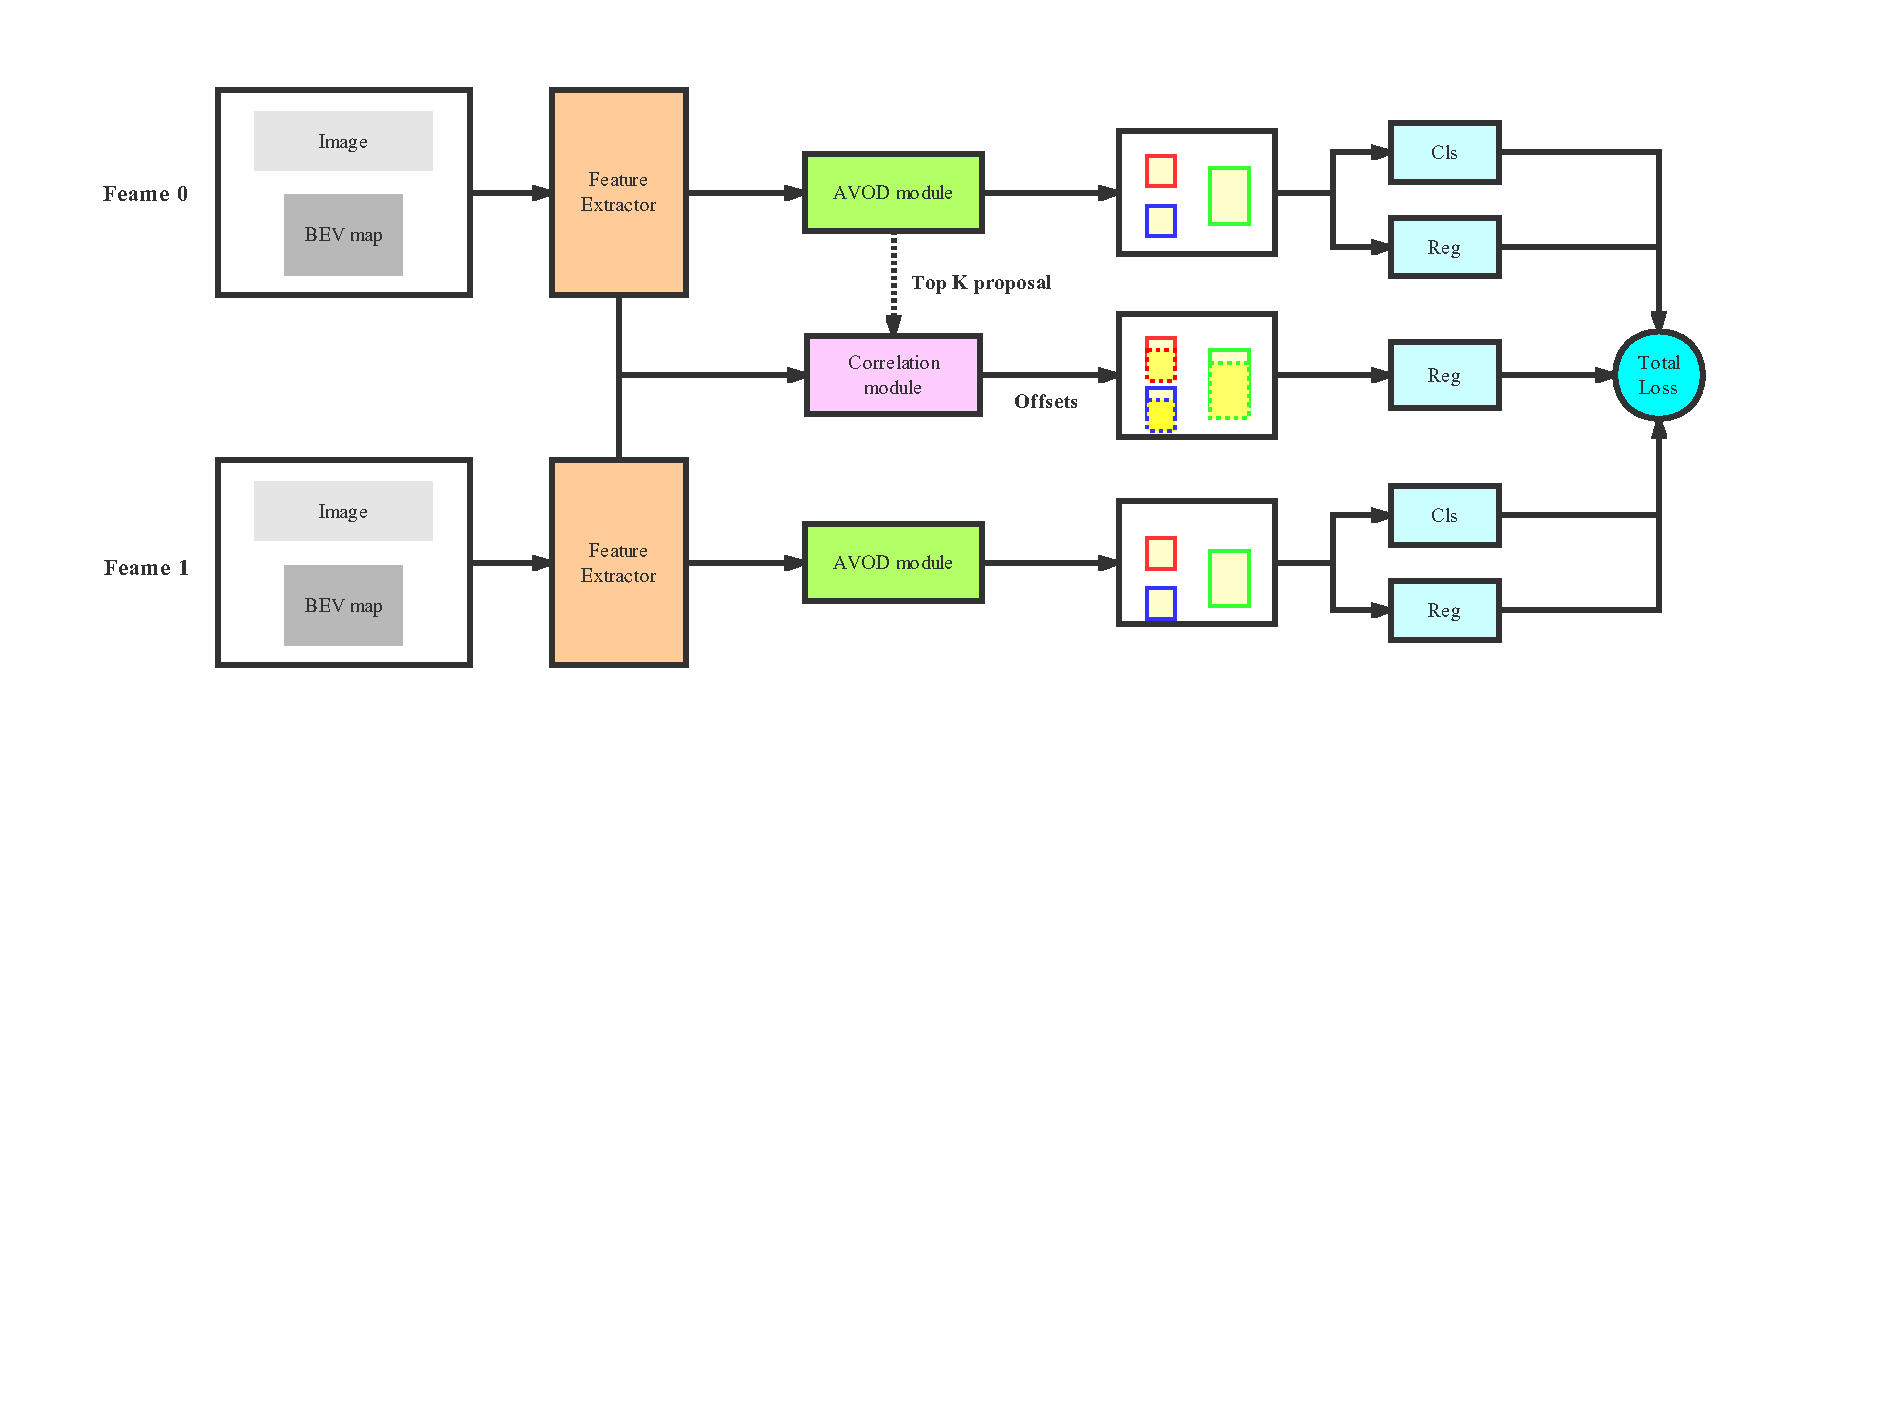
\includegraphics[trim={0cm, 10cm, 3cm, 1cm}, clip, width=\textwidth]{images/Bi-AVOD.pdf}
	\end{center}
	\caption{Bi-AVOD architecture. For convenience, "AVOD module" here does not include feature extractor and loss function.}
	\label{fig:bi-avod}
	\vspace{-0.5cm}
\end{figure}

\begin{figure}
	\setlength{\abovecaptionskip}{-0.5cm}
	\begin{minipage}[t]{0.5\linewidth}
		\centering
		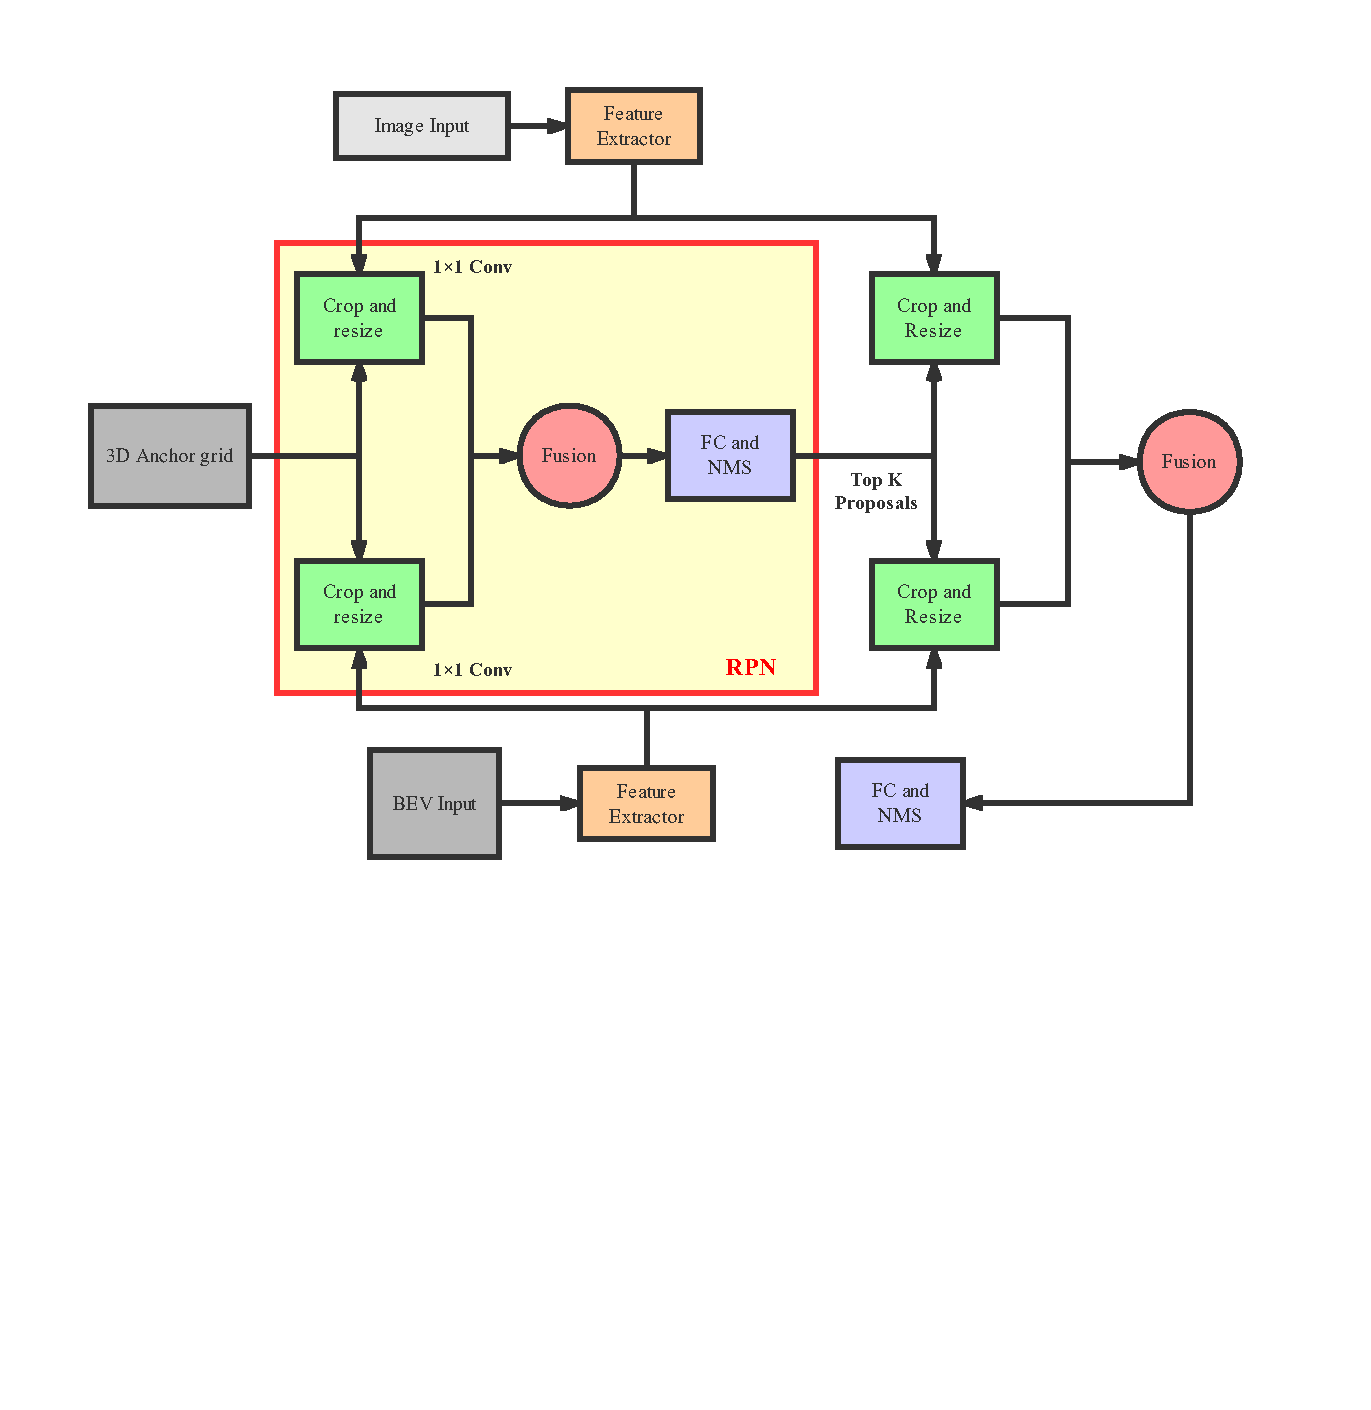
\includegraphics[trim={0cm, 4cm, 2cm, 0cm}, clip, width=2.2in]{images/AVOD.pdf}
		\caption{AVOD architecture}
		\label{fig:avod}
	\end{minipage}%
	\begin{minipage}[t]{0.5\linewidth}
		\centering
		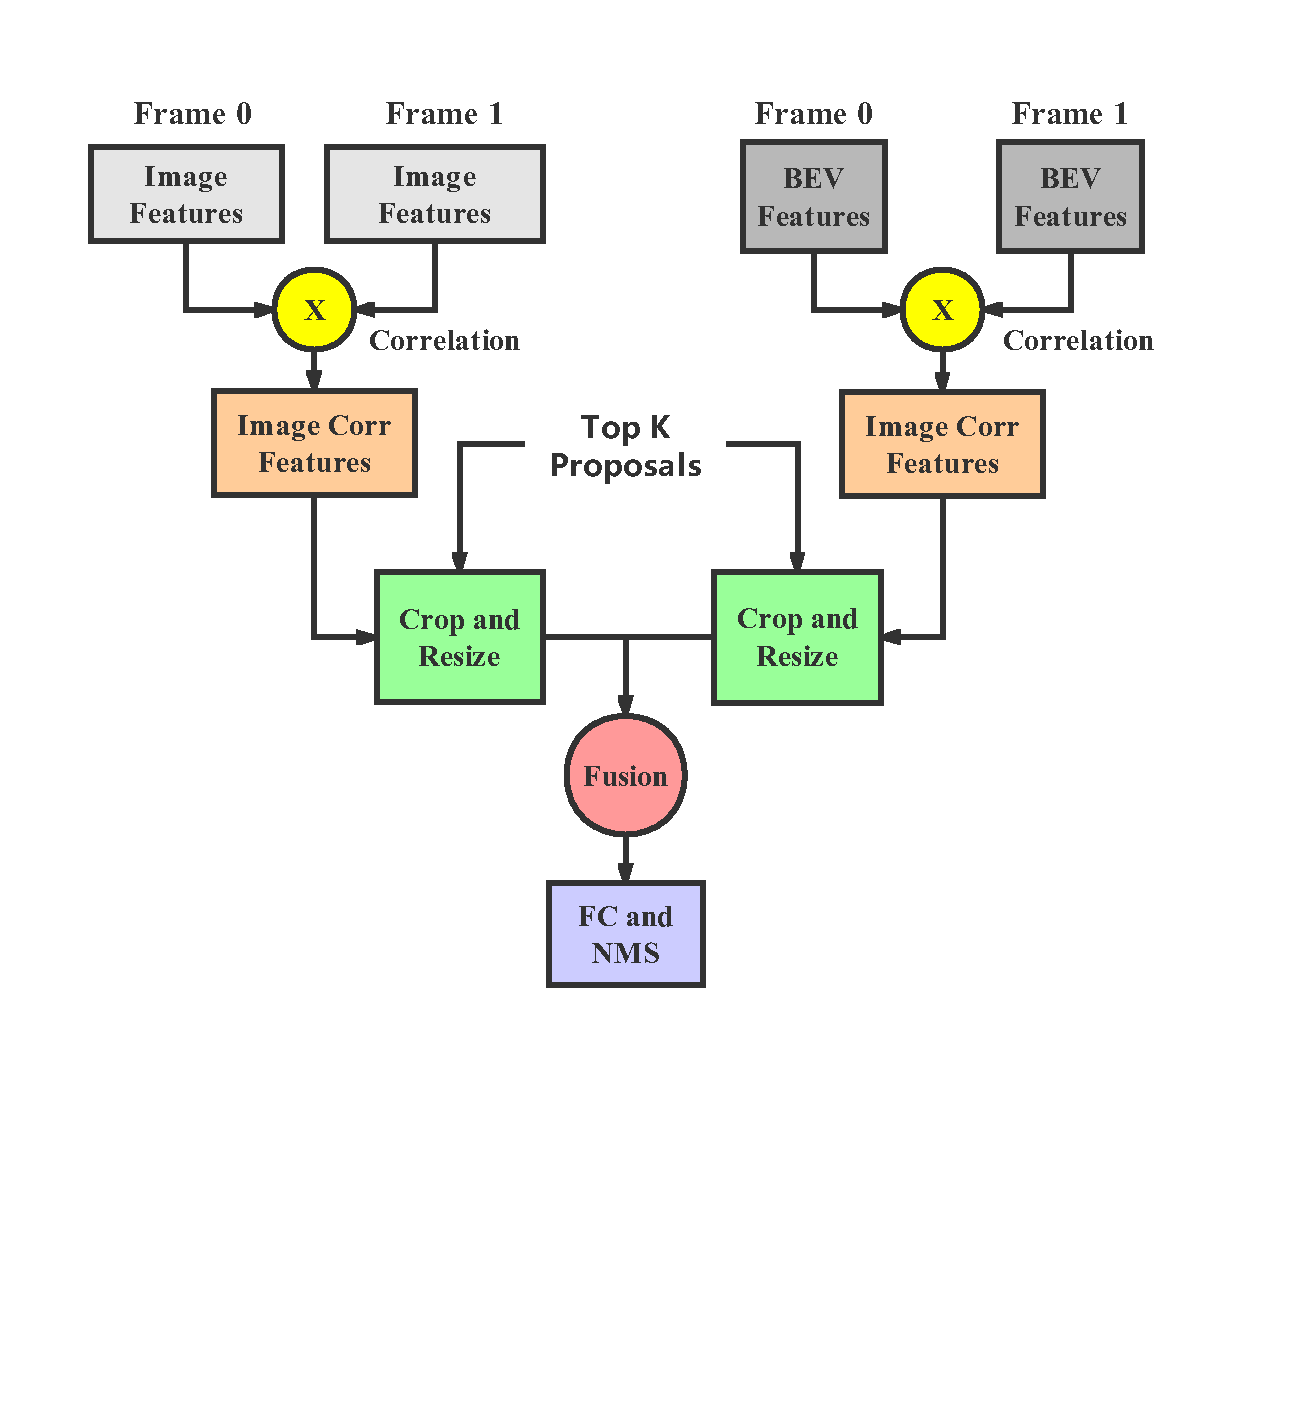
\includegraphics[trim={0cm, 6cm, 2cm, 0cm}, clip, width=2.2in]{images/Correlation.pdf}
		\caption{Correlation module}
		\label{fig:correlation}
	\end{minipage}
\end{figure}

\subsection{Bi-AVOD model structure}
We aim at performing 3D object detection in streaming data, and then apply multi-object tracking using tracking by detection paradigm. We build our Bi-AVOD mainly based on AVOD\cite{ku2018joint}, \figurename .\ref{fig:bi-avod} illustrates our Bi-AVOD architecture. By doubling its input, we can feed two adjacent key frames data (image and point cloud) simultaneously and obtained corresponding object detection results. Meanwhile, the local displacements can be estimated by computing convolutional cross-correlation between the feature responses of adjacent frames using correlation module. With the predicted bounding boxes of two frames and their local displacements, we can perform interpolation algorithms to generate interval bounding boxes for 3D frame-level object detection and develop data association algorithms for 3D object tracking. Note that two \textit{Feature Extractor} and two \textit{AVOD module} in \figurename .\ref{fig:bi-avod} are parameter sharing, thus the increased computational cost comes only from the correlation module. We will simply review the AVOD architecture in this section, and the correlation module will be left to next section.

AVOD architecture in \cite{ku2018joint} is proposed for 3D object detection in autonomous driving by aggregating front view image and bird eye view (BEV) feature maps generated by LiDAR data. It is a two stage method and its architecture is illustrated in \figurename .\ref{fig:avod}. Firstly, it uses feature pyramids based extractors to generate full resolution feature maps from both BEV map and RGB image. Both feature maps are then feed to fusion RPN to generate \textit{Top K} non-oriented region proposals after applied a $1 \times 1$ convolution for dimensionality reduction. Note that the default anchors in image and BEV map are generated through 3D anchor grid projection, and ROI Pooling is implemented by \textit{Crop and Resize} operations. Finally, the \textit{Top K} proposals are passed to the detection network for dimension refinement, orientation estimation and category classification. We refer the reader to \cite{ku2018joint} for an further understanding of the architecture.

\subsection{Correlation module}
The correlation module is illustrated in \figurename .\ref{fig:correlation}. Given feature maps (including image and BEV map) of two adjacent key frames, it first performs correlation operation on two adjacent feature maps to compute convolutional cross-correlation, then similar to the above mentioned RPN in AVOD structure, it extracts feature crops via multiview \textit{Crop and Resize} operations guided by \textit{Top K} non-oriented region proposals which are generated in AVOD module. The feature crops then feed to fusion module and multiview aggregated features are obtained. While the fusion module is identical to the one mentioned in AVOD, which first introduced in MV3D\cite{chen2017multi}, and includes three different fusion schemes, \textit{early fusion}, \textit{late fusion} and \textit{deep fusion}. Finally, the aggregated features are passed to a fully connected layer for regression after performed non-maximum suppression (NMS).

Similar to FlowNet \cite{dosovitskiy2015flownet}, we restrict correlation operation to a local neighborhood instead of all possible circular shifts in a feature map, which avoids large output dimensionality and large targets displacements. The correlation operation performs point-wise feature comparison of two feature maps $f_t$, $f_{t+\tau}$ by

\vspace{-0.5cm}
\begin{equation}
\mathcal{C}^{t, t+\tau}(i, j, p, q) = \Big \langle f_t(i, j), f_{t+\tau} (i+p, j+q) \Big \rangle 
\end{equation}
\vspace{-0.5cm}

where $p, q \in [-d, d]$ are offsets to compared features in a local square window defined by the maximum displacement $d$, and $i, j$ are the location of window center in feature map. The output is a correlation feature map of size $\mathcal{C} \in \mathbb{R}^{h \times w \times (2d+1) \times (2d+1)}$ where $h, w$ are the height, width of the feature map.

After above operation we get two correlation feature maps, one for point cloud $\mathcal{C}^{t, t+\tau}_{pc}$, and another for RGB image $\mathcal{C}^{t, t+\tau}_{img}$. Later ROI pooling and \textit{early fusion} are performed to get aggregate feature $\mathcal{C}^{t,t+\tau}_{fusion} = \frac{1}{2}(\mathcal{C}^{t, t+\tau}_{pc} + \mathcal{C}^{t, t+\tau}_{img})$, which then is flatten and fed to a fully connected layer to predict the transformation
$\Delta^{t, t+\tau} = (\Delta^{t,t+\tau}_{x}, \Delta^{t,t+\tau}_{y}, \Delta^{t,t+\tau}_{z}, \Delta^{t,t+\tau}_{w},  \Delta^{t,t+\tau}_{h},  \Delta^{t,t+\tau}_{l}, \Delta^{t,t+\tau}_{r})$ of the RoIs from $t$ to $t+\tau$. 

\subsection{Multitask detection and correlation objective}
We extend the multi-task loss of object detection, consisting of a classification loss $L_{cls}$ and a regression loss $L_{reg}$, with an additional term $L_{corr}$ that scores the displacement regression between corresponding objects across two frames. Considering a batch of $N$ RoIs after category balanced sampling, the network predicts softmax probabilities $\{p_i\}^N_{i=1}$, bounding box regression offsets $\{b_i\}^N_{i=1}$, and cross-frame displacement regression $\{\Delta^{t+\tau}_i\}^{N_{corr}}_{i=1}$, the overall objective function is shown as:

\vspace{-0.5cm}
\begin{equation}
\begin{split}
L(\{p_i\}, \{b_i\}, \{\Delta_i\}) = \frac{1}{N} \sum^N_{i=1} L_{cls}(p_{i, c^*}) 
+ \frac{\alpha}{N_{fg}}\sum^N_{i=1} [c^*_i > 0]L_{reg}(b_i, b^*_i) \\
+ \frac{\beta}{N_{corr}} \sum^{N_{corr}}_{i=1}L_{corr}(\Delta^{t+\tau}_i, \Delta^{*, t+\tau}_i)
\end{split}
\end{equation}
\vspace{-0.3cm}

where $c^*_i$ is the ground truth class label of an RoI and $p_{i, c^*_i}$ is corresponding predicted softmax score. $b^*_i$ is the ground truth of bounding box regression target, and $\Delta^{*, t+\tau}_i$ is the ground truth of displacement regression target. The indicator function $ [c^*_i > 0]$ is 1 for foreground RoIs and 0 for background RoIs. $L_{cls}$ is cross-entropy loss, and $L_{reg}$, $L_{corr}$ are smooth L1 loss \cite{girshick2015fast}. $\alpha$ and $\beta$ are weight coefficients for $L_{reg}$ and $L_{corr}$, in this work we set 5 and 1 respectively. Note that we only consider the $N_{fg}$ foreground RoIs loss for $L_{reg}$, and $L_{corr}$ is active only for foreground RoIs which have a track correspondence in both two key frames. Additionally, $b^*_i$ and $ \Delta^{*, t+\tau}_i$ are all encoded following the method in \cite{ku2018joint}.

\subsection{3D streaming object detection and tracking}
Give a sequence of $N$ frames $\{I_f\}$ for $f \in \{1, ... N\}$, the streaming object detection task needs to predict a set of bounding boxes $D_f$ for each frame $I_f$. Each set $D_f$ consists of object detections $\{D^i_f\}$ while $i \in \{1,...N_f\}$ ($N_f$ is the number of targets in frame $f$). Note that $D_f$ can also be an empty set when no target is detected in a frame. In 3D object detection, Each detection $D^i_f$ is parametrized as $D^i_f = (x^i_f, y^i_f, z^i_f, w^i_f, h^i_f, l^i_f, \theta^i_f, s^i_f)$, where $(x^i_f, y^i_f, z^i_f)$ corresponds to the coordinate of target center, $(w^i_f, h^i_f, l^i_f)$ corresponds to width, height, length of the target, $\theta^i_f$ is the rotation angle in yaw axis and $s^i_f$ is prediction confidence of the target.

Because of the redundant features in streaming, we only need to perform object detection in key frames, while the bounding boxes of the intermediate frames can be determined leveraging the detection results of adjacent two key frames. Support we have two predicted object bounding boxes set $(D_f, D_{f+\tau})$ of two consecutive key frames $(I_f, I_{f+\tau})$, where $\tau$ is temporal stride, the detection results $\{D^i_{f+t}\}$ $(t \in \{1, \tau-1\})$ of intermediate frame $I_{f+t}$ can be obtained by

\begin{equation}
D^i_{f+t} = \mathcal{F}(W_f D^i_f, W_{f+\tau} D^i_{f+\tau})
\end{equation}

where $W_f, W_{f+\tau}$ is corresponding weight coefficients and $\mathcal{F}$ is interpolation function to produce $D^i_{f+t}$, in this paper we simply use linear interpolation. Note that we can use (1) to generate $D^i_{f+t}$ only when the target exists in $D_f$ and $D_{f+\tau}$ simultaneously. If the target is start or end in intermediate frames, this method would be failed. Though we can develop the key frames selection algorithm carefully to avoid this problem, it is beyond the scope of this article. In this paper we focus on the targets that always exist between two key frames.

With object detection result of each frame, multi-object tracking can be implemented using tracking-by-detection paradigm. For each predicted bounding box in every frame, we try to associate it to a unique target trajectory $T_k = \{D^k_{f_1}, D^k_{f_2}, ..., D^k_{f_{N_k}}\}$ utilizing extending IOU tracker algorithm \cite{bochinski2018extending}, where $k$ is trajectory id and $N_k$ is the length of $T_k$, $\{f_1, f_2, ..., f_{N_k}\}$ are corresponding frames id. Unlike multi-object tracking in 2D image that suffers from boxes overlap, bounding box in 3D has its unique position and any overlap in 3D of two bounding boxes means high probability of the same target, thus a simply IOU based tracking algorithm can also perform well.

%-------------------------------------------------------------------------
\section{Experimental evaluation}
\label{sec:experiments}

\subsection{Datasets}
We use the KITTI object tracking Benchmark \cite{geiger2013vision} for evaluation. It consists of 21 training sequences and 29 test sequences with vehicles annotated in 3D. Each sequence includes hundreds of point clouds frames captured by Velodyne HDL-64E rotating 3D laser scanner and corresponding RGB images. We split 21 training sequences into two parts based on the parity of the sequence number, odd number for training and even number for evaluation. For multi-object tracking evaluation, we train our model in all 21 training sequences.

\subsection{Training}

\textbf{Datasets preprocessing.} Like other work based on KITTI datasets, the point cloud is cropped at $[-40, 40] \times [0, 70] \times [0, 2.5]$ meters along $Y, X, Z$ axis respectively to contain points within the field of view of the camera. In KITTI tracking datasets, the observer is an autonomous vehicle, thus the coordinate system of two frames would be shifted due to the moving of the observer over time. Since the location and velocity information of each frame are available in its IMU data, one can calculate the displacement of the observer between different frames and translate the coordinates accordingly. By this way both point clouds and object labels are on the exact same coordinate system. Note that this approach is important to make the system invariant to the speed of the ego-car.

\textbf{Training and testing.} We train two networks, one for the \textit{Car} class and another for both \textit{Pedestrian} and \textit{Cyclist} classes. We follow most of the super-parameter settings in AVOD\cite{ku2018joint} during training and testing. To be more specific, the network is trained for 120K iterations using an ADAM\cite{kingma2014adam} optimizer with an initial learning rate of 0.0001 that is decayed exponentially every 30K iterations with a decay factor of 0.8. During proposal generation, anchors with IoU less than 0.3 are considered background and greater than 0.5 are object anchors for \textit{Car}. For \textit{Pedestrian} and \textit{Cyclist} classes, the IoU thresholds are 0.3 and 0.45 respectively. To remove redundant proposals, we perform 2D non-maximum suppression(NMS) at an IoU threshold of 0.8 in BEV to keep the top 1024 proposals during training, while at inference time, top 300 proposals are used for \textit{Car} class and top 1024 proposals are kept for \textit{Pedestrian} and \textit{Cyclist} class.

\subsection{Results}

\textbf{3D object detection.} Our work mainly based on 3D object detection, either streaming level detection or multi-object tracking, thus the network performance on 3D object detection is significant important. We train our Bi-AVOD on KITTI tracking datasets, and results are evaluated using KITTI object detection metrics. Since there is no way for us to evaluate object detection performance on KITTI tracking testing datasets, we evaluate our Bi-AVOD on tracking evaluation datasets (described in Sec 4.1) instead. To explore the effectiveness of dual-way structure on object detection, we train original AVOD model on tracking datasets for comparison, results are shown in \tablename \, \ref{table:result_detection}. Our Bi-AVOD model is shown to have comparable ability for \textit{easy, moderate, hard} setting on all three classes. This means that the introduction of dual-way model and correlation operation do not reduce model performance on 3D object detection. In pursuit of better network performance, we pre-trained original AVOD model on KITTI object detection datasets, and then migrated relevant parameters to our Bi-AVOD model for further fine-tuned learning on KITTI tracking datasets. By this way a better performance is obtained and results are shown in \tablename \, \ref{table:result_detection}, where Bi-AVOD* is the fine-tuned model. Compared to Bi-AVOD which trained from scratch, the fine-tuned model outperform by 5.20\% AP on the \textit{moderate} setting and 4.05\% on the \textit{hard} setting respectively. 

\begin{table}[]\centering
	\footnotesize
	\begin{tabular}{ccccccccc}
				 &   		   &  											& \multicolumn{3}{c}{$AP_{3D}(\%)$}  		 & \multicolumn{3}{c}{$AP_{BEV}(\%)$} \\ \toprule[1.5pt]
		Method   & Runtime (s) & \multicolumn{1}{c|}{Class}  				& Easy & Moderate & \multicolumn{1}{c|}{Hard} & Easy    & Moderate    & Hard    \\ \midrule
		AVOD     & 0.01        & \multicolumn{1}{c|}{\multirow{3}{*}{Car}}  & 0.90 & 0.80     & \multicolumn{1}{c|}{0.70} & 0.80    & 0.70        & 0.60    \\
		Bi-AVOD  & 0.01        & \multicolumn{1}{c|}{}                      & 0.90 & 0.80     & \multicolumn{1}{c|}{0.70} & 0.80    & 0.70        & 0.60    \\
		Bi-AVOD* & 0.01        & \multicolumn{1}{c|}{}                      & 0.90 & 0.80     & \multicolumn{1}{c|}{0.70} & 0.80    & 0.70        & 0.60    \\ \midrule
		AVOD     & 0.01        & \multicolumn{1}{c|}{\multirow{3}{*}{Ped.}} & 0.90 & 0.80     & \multicolumn{1}{c|}{0.70} & 0.80    & 0.70        & 0.60    \\
		Bi-AVOD  & 0.01        & \multicolumn{1}{c|}{}                      & 0.90 & 0.80     & \multicolumn{1}{c|}{0.70} & 0.80    & 0.70        & 0.60    \\
		Bi-AVOD* & 0.01        & \multicolumn{1}{c|}{}                      & 0.90 & 0.80     & \multicolumn{1}{c|}{0.70} & 0.80    & 0.70        & 0.60    \\ \midrule
		AVOD     & 0.01        & \multicolumn{1}{c|}{\multirow{3}{*}{Cyc.}} & 0.90 & 0.80     & \multicolumn{1}{c|}{0.70} & 0.80    & 0.70        & 0.60    \\
		Bi-AVOD  & 0.01        & \multicolumn{1}{c|}{}                      & 0.90 & 0.80     & \multicolumn{1}{c|}{0.70} & 0.80    & 0.70        & 0.60    \\
		Bi-AVOD* & 0.01        & \multicolumn{1}{c|}{}                      & 0.90 & 0.80     & \multicolumn{1}{c|}{0.70} & 0.80    & 0.70        & 0.60    \\
		\bottomrule[1.5pt]
	\end{tabular}
	\setlength{\abovecaptionskip}{1pt}
	\caption{A comparison of the performance between original AVOD, our Bi-AVOD and fine-tuned Bi-AVOD* on KITTI tracking evaluation datasets.}
	\label{table:result_detection}
\end{table}

\begin{table}[]\centering
	\footnotesize
	\begin{tabular}{ccccccccc}
		&   		   &  											& \multicolumn{3}{c}{$AP_{3D}(\%)$}  		 & \multicolumn{3}{c}{$AP_{BEV}(\%)$} \\ \toprule[1.5pt]
		Method                & Runtime (s) & \multicolumn{1}{c|}{Class}  				& Easy & Moderate & \multicolumn{1}{c|}{Hard} & Easy    & Moderate    & Hard    \\ \midrule
		AVOD                  & 0.01        & \multicolumn{1}{c|}{\multirow{4}{*}{Car}}  & 0.90 & 0.80     & \multicolumn{1}{c|}{0.70} & 0.80    & 0.70        & 0.60    \\
		Bi-AVOD ($\tau$ = 1)  & 0.01        & \multicolumn{1}{c|}{}                      & 0.90 & 0.80     & \multicolumn{1}{c|}{0.70} & 0.80    & 0.70        & 0.60    \\
		Bi-AVOD ($\tau$ = 3)  & 0.01        & \multicolumn{1}{c|}{}                      & 0.90 & 0.80     & \multicolumn{1}{c|}{0.70} & 0.80    & 0.70        & 0.60    \\
		Bi-AVOD ($\tau$ = 5)  & 0.01        & \multicolumn{1}{c|}{}                      & 0.90 & 0.80     & \multicolumn{1}{c|}{0.70} & 0.80    & 0.70        & 0.60    \\ \midrule
		AVOD                  & 0.01        & \multicolumn{1}{c|}{\multirow{4}{*}{Ped.}} & 0.90 & 0.80     & \multicolumn{1}{c|}{0.70} & 0.80    & 0.70        & 0.60    \\
		Bi-AVOD ($\tau$ = 1)  & 0.01        & \multicolumn{1}{c|}{}                      & 0.90 & 0.80     & \multicolumn{1}{c|}{0.70} & 0.80    & 0.70        & 0.60    \\
		Bi-AVOD ($\tau$ = 3)  & 0.01        & \multicolumn{1}{c|}{}                      & 0.90 & 0.80     & \multicolumn{1}{c|}{0.70} & 0.80    & 0.70        & 0.60    \\
		Bi-AVOD ($\tau$ = 5)  & 0.01        & \multicolumn{1}{c|}{}                      & 0.90 & 0.80     & \multicolumn{1}{c|}{0.70} & 0.80    & 0.70        & 0.60    \\ \midrule
		AVOD                  & 0.01        & \multicolumn{1}{c|}{\multirow{4}{*}{Cyc.}} & 0.90 & 0.80     & \multicolumn{1}{c|}{0.70} & 0.80    & 0.70        & 0.60    \\
		Bi-AVOD ($\tau$ = 1)  & 0.01        & \multicolumn{1}{c|}{}                      & 0.90 & 0.80     & \multicolumn{1}{c|}{0.70} & 0.80    & 0.70        & 0.60    \\
		Bi-AVOD ($\tau$ = 3)  & 0.01        & \multicolumn{1}{c|}{}                      & 0.90 & 0.80     & \multicolumn{1}{c|}{0.70} & 0.80    & 0.70        & 0.60    \\
		Bi-AVOD ($\tau$ = 5)  & 0.01        & \multicolumn{1}{c|}{}                      & 0.90 & 0.80     & \multicolumn{1}{c|}{0.70} & 0.80    & 0.70        & 0.60    \\
		\bottomrule[1.5pt]
	\end{tabular}
	\setlength{\abovecaptionskip}{1pt}
	\caption{Performance comparison of different temporally strides $\tau$ during testing.}
	\label{table:result_streaming}
\end{table}

\textbf{Streaming level detection.} Using accurate 3D object detection results of adjacent key frames and corresponding targets displacements, we can perform streaming level 3D object detection on autonomous driving scenarios. This part we investigate the effect of multi-frame input during testing, specifically, we focus on the influence on time and precise of different temporally strides $\tau$. In \tablename \, \ref{table:result_streaming} we see that linking detections to tubes based on corresponding targets displacements results in speed and precision improvements more or less. This gain is mostly for the following reason: if a bounding box is false negative in intermediate frame but is true positive in its two adjacent frames, it will be corrected during linking; on the other hand, a false positive predicted box will be modified to true positive if it considered as true bounding box in its adjacent frames. Note that a large $\tau$ will leads to a remarkable speed but a significant accuracy decay in detection, there is a treat-off between runtime and precision. Our experiments show that $\tau = 3$ is the best choice on KITTI tracking datasets.

\begin{figure*}
	\rule{0pt}{1ex}
	\setlength{\abovecaptionskip}{-0.5cm}
	\begin{center}
		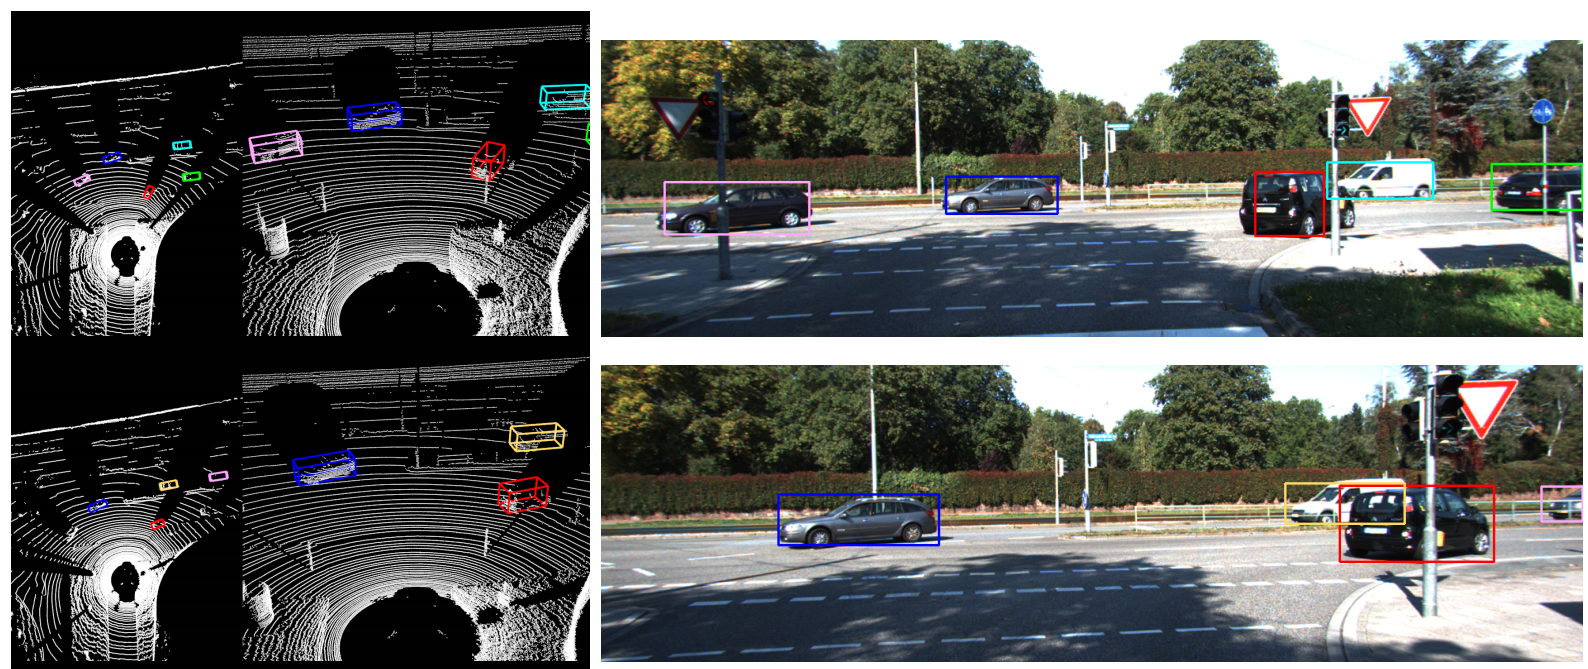
\includegraphics[width=\textwidth]{images/examples.png}
	\end{center}
	\caption{\textbf{Need to be updated}. Visualization of a set of trajectories produced by the tracker over 15 frames. Trajectories are color coded, such that
				having the same color means it's the same object.}
	\label{fig:examples}
	\vspace{-0.5cm}
\end{figure*}

\textbf{Multi-object tracking.} We finally validate the efficacy of our Bi-AVOD network on multi-object tracking task. We compare our model to publicly available methods in the KITTI Tracking Benchmark, the results are listed in \tablename \, \ref{label:result_tracking}. It's shown that our approach is competitive with the start-of-the-art, outperforming all other methods in some of the metrics (best for MOTP and MT, second best for ML) by a large margin. Note that KITTI only evaluates the metrics in 2D, which does not fully represent the performance of our 3D approach. Also we refer the reader to \figurename .\ref{fig:examples} for an visualization example of the multi-object tracking results, more examples are available in Supplementary material.
\begin{table}[]\centering
	\footnotesize
	\begin{tabular}{ccccccc}
		\toprule[1.5pt]
		Method        & MOTA(\%) & MOTP(\%) & MT(\%) & ML(\%) & IDS & FRAG \\ \midrule
		CEM           & 51.94    & 77.11    & 20.00  & 31.54  & 125 & 396  \\
		RMOT          & 52.42    & 75.18    & 21.69  & 31.85  & 50  & 376  \\
		TBD           & 55.07    & 78.35    & 20.46  & 32.62  & 31  & 529  \\
		mbodSSP       & 56.03    & 77.52    & 23.23  & 27.23  & 0   & 699  \\
		SCEA          & 57.03    & 78.84    & 26.92  & 26.62  & 17  & 461  \\
		SSP           & 57.85    & 77.64    & 29.38  & 24.31  & 7   & 704  \\
		ODAMOT        & 59.23    & 75.45    & 27.08  & 15.54  & 389 & 1274 \\
		NOMT-HM       & 61.17    & 78.65    & 33.85  & 28.00  & 28  & 241  \\
		LP-SSVM       & 61.77    & 76.93    & 35.54  & 21.69  & 16  & 422  \\
		RMOT*         & 65.83    & 75.42    & 40.15  & 9.69   & 209 & 727  \\
		NOMT          & 66.60    & 78.17    & 41.08  & 25.23  & 13  & 150  \\
		DCO-X*        & 68.11    & 78.85    & 37.54  & 14.15  & 318 & 959  \\
		mbodSSP*      & 72.69    & 78.75    & 48.77  & 8.77   & 114 & 858  \\
		SSP*          & 72.72    & 78.55    & 53.85  & 8.00   & 185 & 932  \\
		NOMT-HM*      & 75.20    & 80.02    & 50.00  & 13.54  & 105 & 351  \\
		SCEA*         & 75.58    & 79.39    & 53.08  & 11.54  & 104 & 448  \\
		MDP           & 76.59    & 82.10    & 52.15  & 13.38  & 130 & 387  \\
		LP-SSVM*      & 77.63    & 77.80    & 56.31  & 8.46   & 62  & 539  \\
		NOMT*         & 78.15    & 79.46    & 57.23  & 13.23  & 31  & 207  \\
		MCMOT-CPD     & 78.90    & 82.13    & 52.31  & 11.69  & 228 & 536  \\
		DSM           & 76.15    & 83.42    & 60.00  & 8.31   & 296 & 868  \\ \midrule
		Bi-AVOD(ours) & 80.00    & 90.00    & 70.00  & 8.00   & 200 & 500  \\ 
		\bottomrule[1.5pt]
	\end{tabular}
	\setlength{\abovecaptionskip}{1pt}
	\caption{Tracking performance comparison of publicly available methods in the KITTI Tracking Benchmark.}
	\label{label:result_tracking}
\end{table}


%-------------------------------------------------------------------------
\section{Conclusions}
\label{sec:conclusions} In this work we proposed Bi-AVOD, a unified framework for simultaneous 3D object detection and tracking in 3D streaming data. The network is a dual-way structure and can  process two frames at a same time, which makes multi-frame detection possible. Meanwhile, embedding with a correlation module to encode the similarity and diversity of adjacent frames, our network can do object detection and tracking in a very efficient way. In multi-object tracking evaluation, our approach achieves accuracy competitive state-of-the-art methods with a higher speed. In the future, we plan to improve our approach with an adaptive key frame selection algorithm.

%-------------------------------------------------------------------------
\bibliography{egbib}
\end{document}
